\subsection{Business Layer}

\begin{figure}[H]
    \centering
    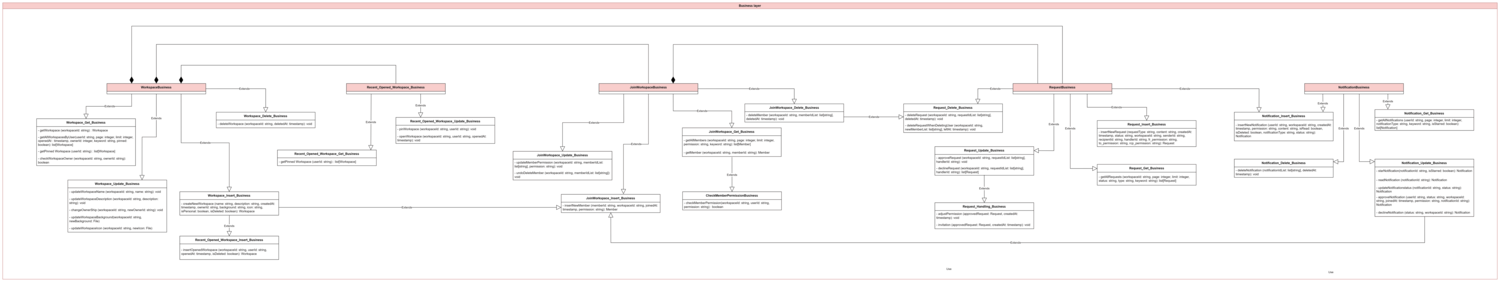
\includegraphics[ width = \linewidth]{Content/Phân tích và thiết kế hệ thống/documents/Sơ đồ lớp/images/Business layer/businessLayer.png}
    \vspace{0.5cm}
    \caption{Tổng quan Business Layer}
    \label{fig:Tổng quan Business Layer}
\end{figure}

Nhiệm vụ của tầng Business là phân tích những yêu cầu, xử lý logic nghiệp vụ và
gọi tới các đối tượng ở tầng Persistence để tương tác với cơ sở dữ liệu.

\begin{figure}[H]
    \centering
    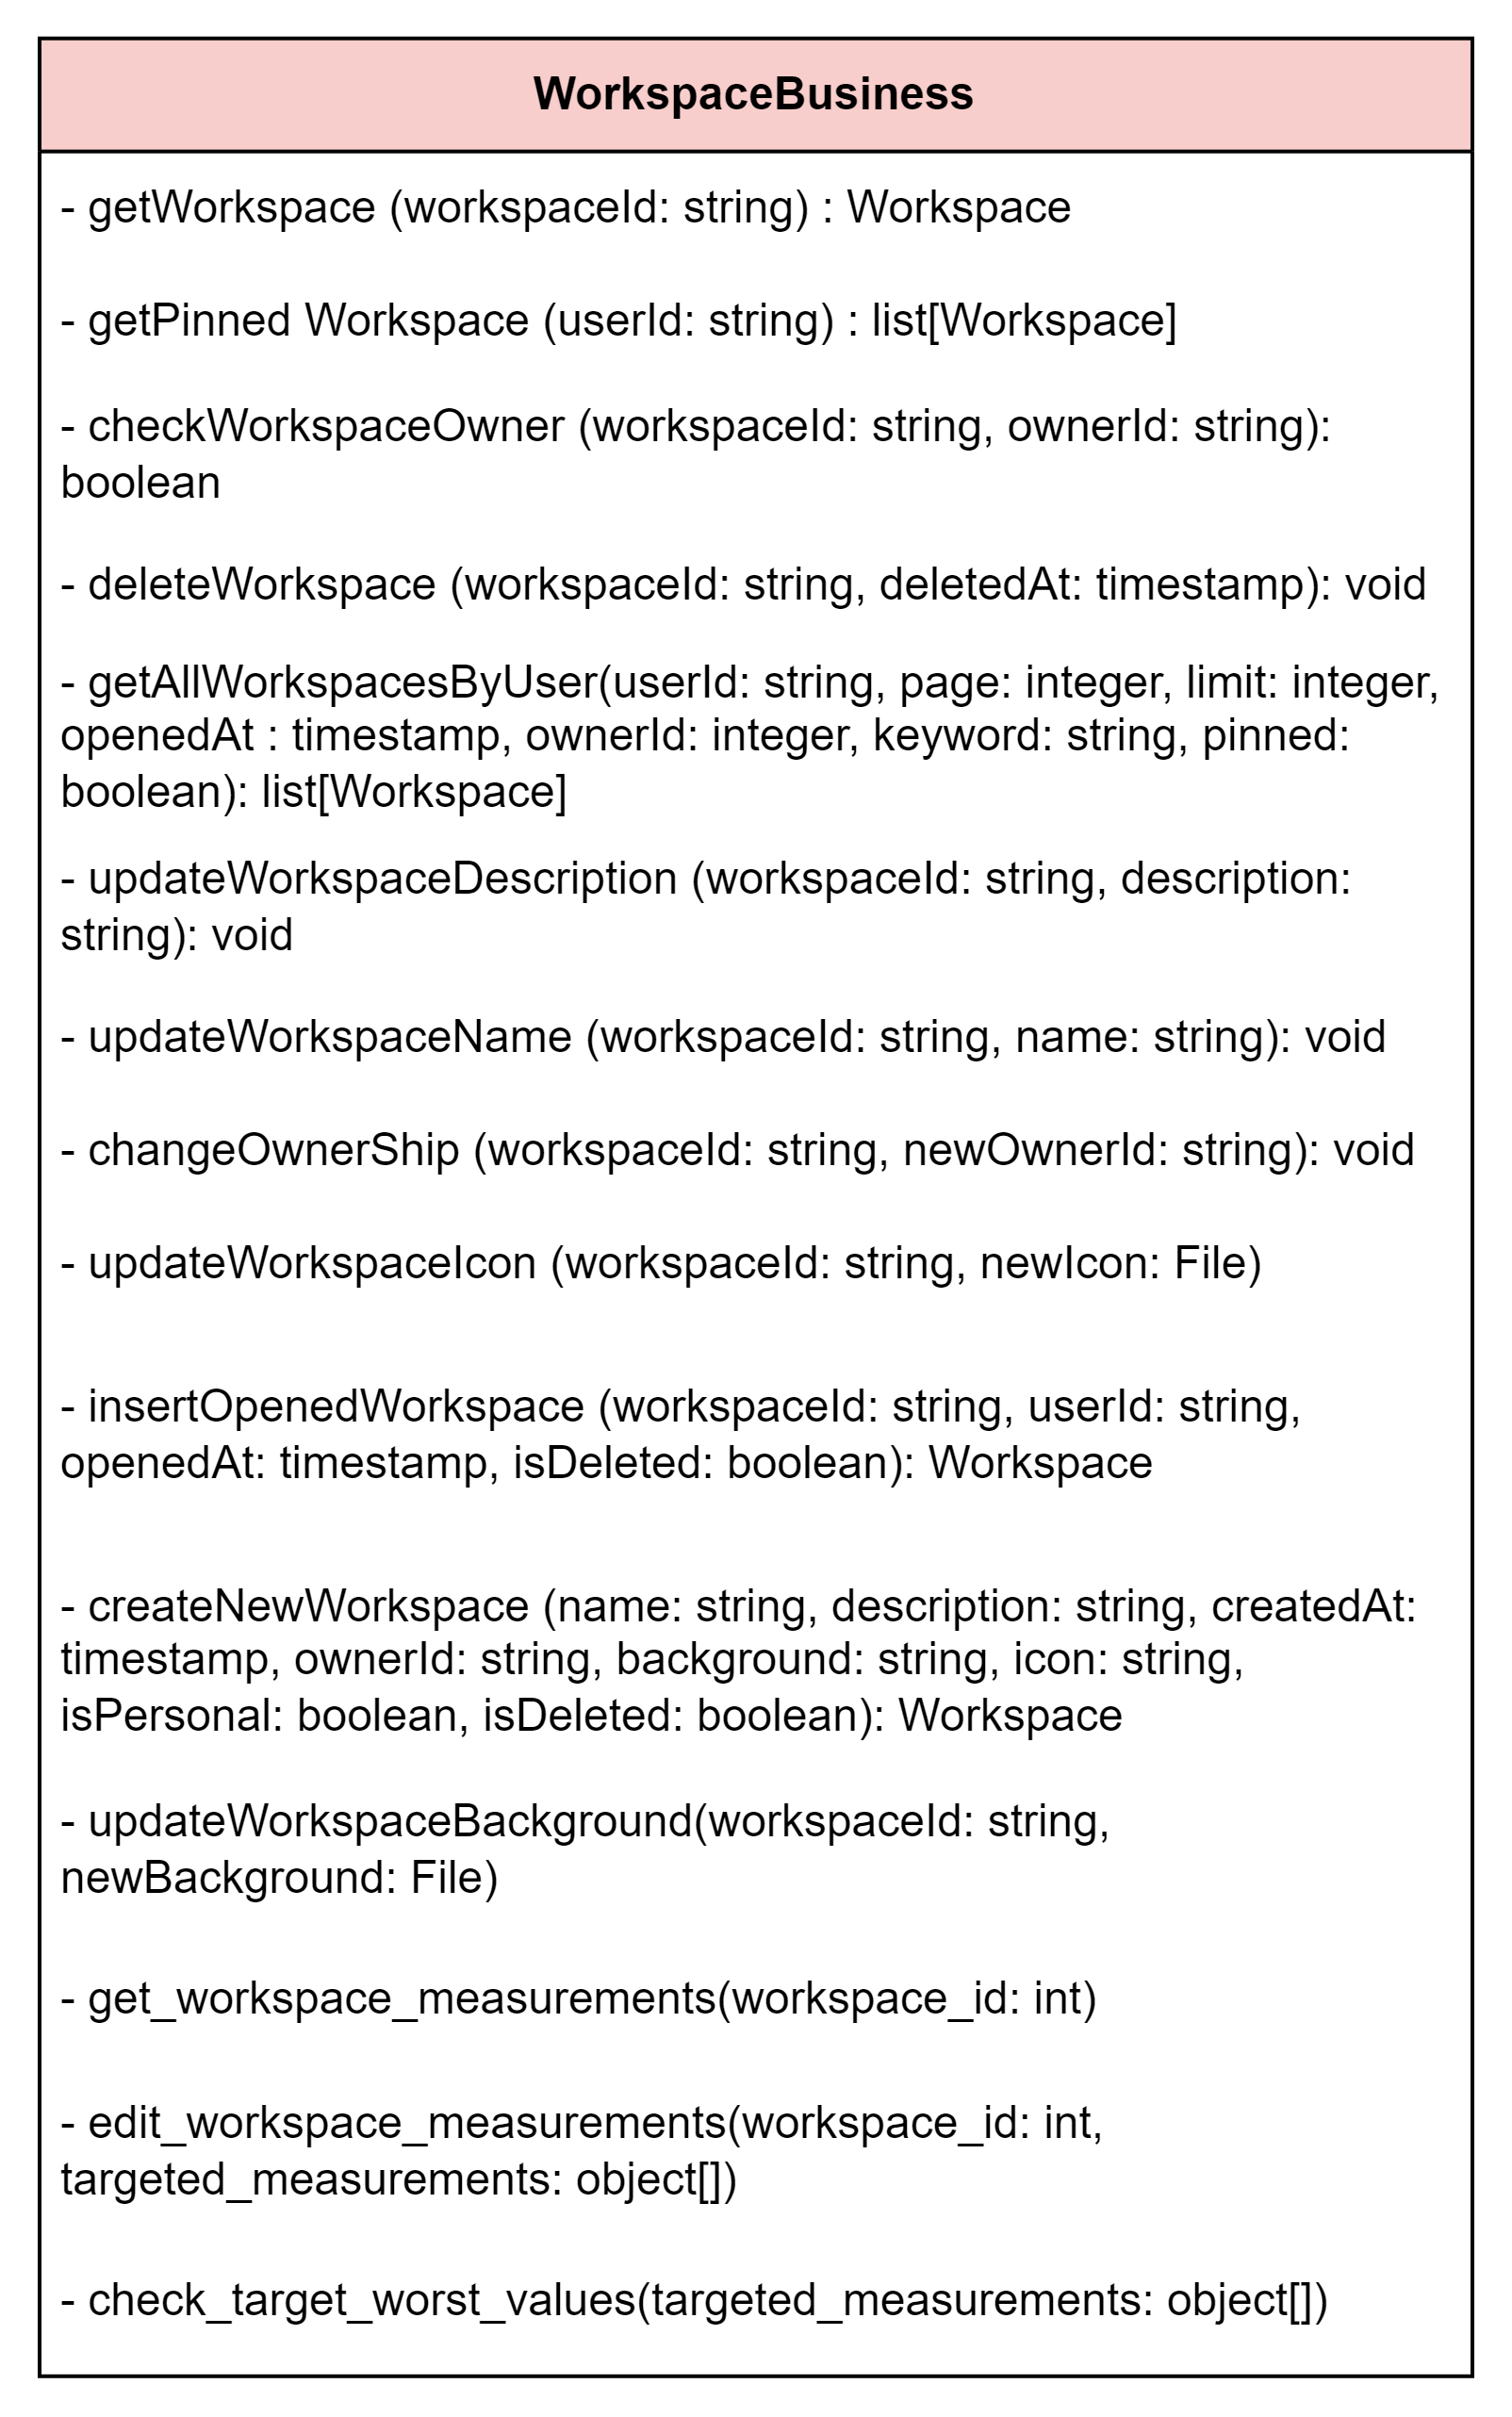
\includegraphics[ width = \linewidth]{Content/Phân tích và thiết kế hệ thống/documents/Sơ đồ lớp/images/Business layer/workspaceBusiness.png}
    \vspace{0.5cm}
    \caption{Class WorkspaceBusiness trong Business layer}
    \label{fig:Class WorkspaceBusiness trong Business layer}
\end{figure}

\par
Class WorkspaceBusiness là class chịu trách nhiệm xử lý logic nghiệp vụ liên quan
đến Workspace. Class này sẽ thừa kế các class khác như: Workspace\_Get\_Business,
Workspace\_Delete\_Business, Workspace\_Update\_Business, Workspace\_Insert\_Business.
Những class này sẽ thực hiện các chức năng tương ứng với tên của chúng, như vậy,
bằng cách này sẽ giúp cho việc quản lý code dễ dàng hơn, và khi có sự thay đổi
trong một chức năng nào đó thì việc thay đổi này sẽ không ảnh hưởng đến các chức
năng khác. Ngoài ra, class Workspace\_Insert\_Business còn thừa kế class
Recent\_Opened\_Workspace\_Insert\_Business để thực hiện chức năng thêm mới vào 
bảng Recent\_Opened\_Workspace.
\begin{figure}[H]
    \centering
    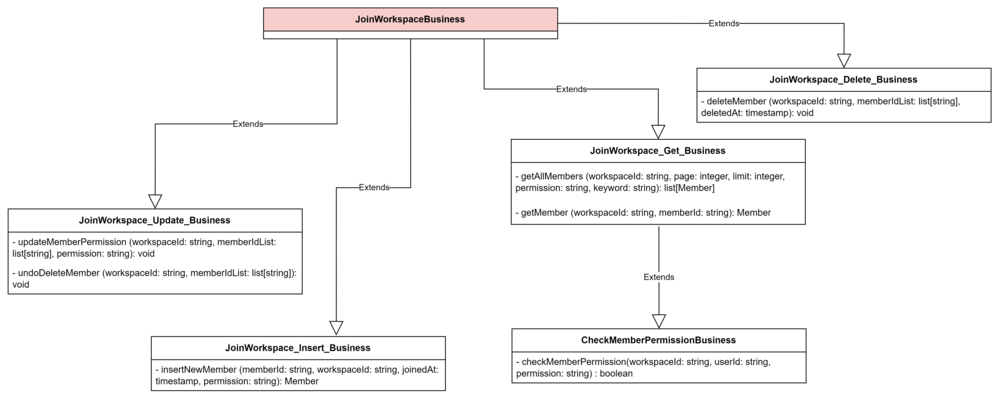
\includegraphics[ width = \linewidth]{Content/Phân tích và thiết kế hệ thống/documents/Sơ đồ lớp/images/Business layer/joinWorkspaceBusiness.png}
    \vspace{0.5cm}
    \caption{Class JoinWorkspaceBusiness trong Business layer}
    \label{fig:Class JoinWorkspaceBusiness trong Business layer}
\end{figure}
\par
Class Join\_Workspace\_Business là class chịu trách nhiệm xử lý logic nghiệp vụ liên quan đến
việc người dùng tham gia vào một Workspace. Class này sẽ thừa kế các class khác như:
Join\_Workspace\_Get\_Business, Join\_Workspace\_Delete\_Business, Join\_Workspace\_Update\_Business.
Những class này sẽ thực hiện các chức năng tương ứng với tên của chúng. Ngoài ra, class
JoinWorkspace\_Get\_Business còn kế thừa từ class CheckMemberPermissionBusiness để thực hiện
chức năng kiểm tra quyền của người dùng trong một Workspace.
\begin{figure}[H]
    \centering
    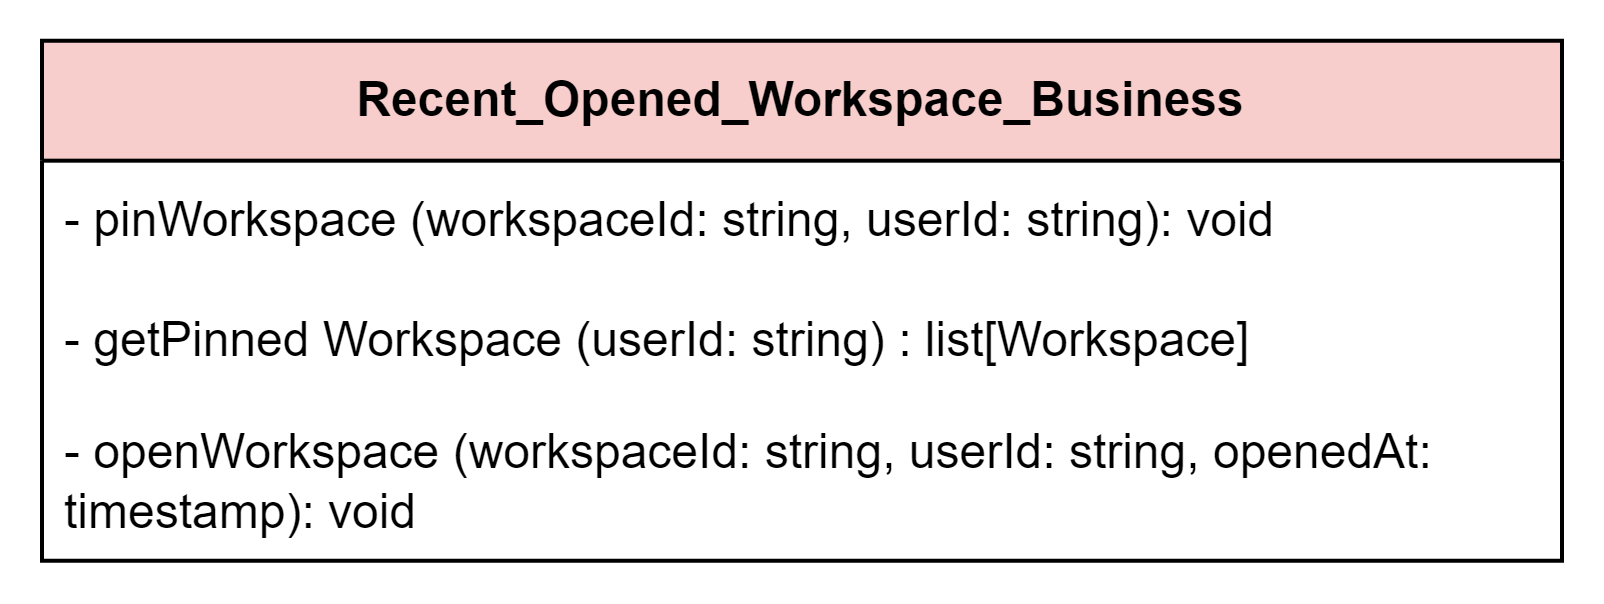
\includegraphics[ width = \linewidth]{Content/Phân tích và thiết kế hệ thống/documents/Sơ đồ lớp/images/Business layer/recentOpenedWorkspaceBusiness.png}
    \vspace{0.5cm}
    \caption{Class RecentOpenedWorkspaceBusiness trong Business layer}
    \label{fig:Class RecentOpenedWorkspaceBusiness trong Business layer}
\end{figure}
\par
Class Recent\_Opened\_Workspace\_Business là class chịu trách nhiệm xử lý logic
cho nghiệp vụ liên quan đến những workspace được mở gần đây của người dùng.
Class này chỉ kế thừa hai class khác: Recent\_Opened\_Workspace\_Get\_Business và
Recent\_Opened\_Workspace\_Update\_Business cho những xử lý logic khi lấy danh sách 
Workspace được đánh dấu và logic mở cũng như đánh dấu một Workspace.
\begin{figure}[H]
    \centering
    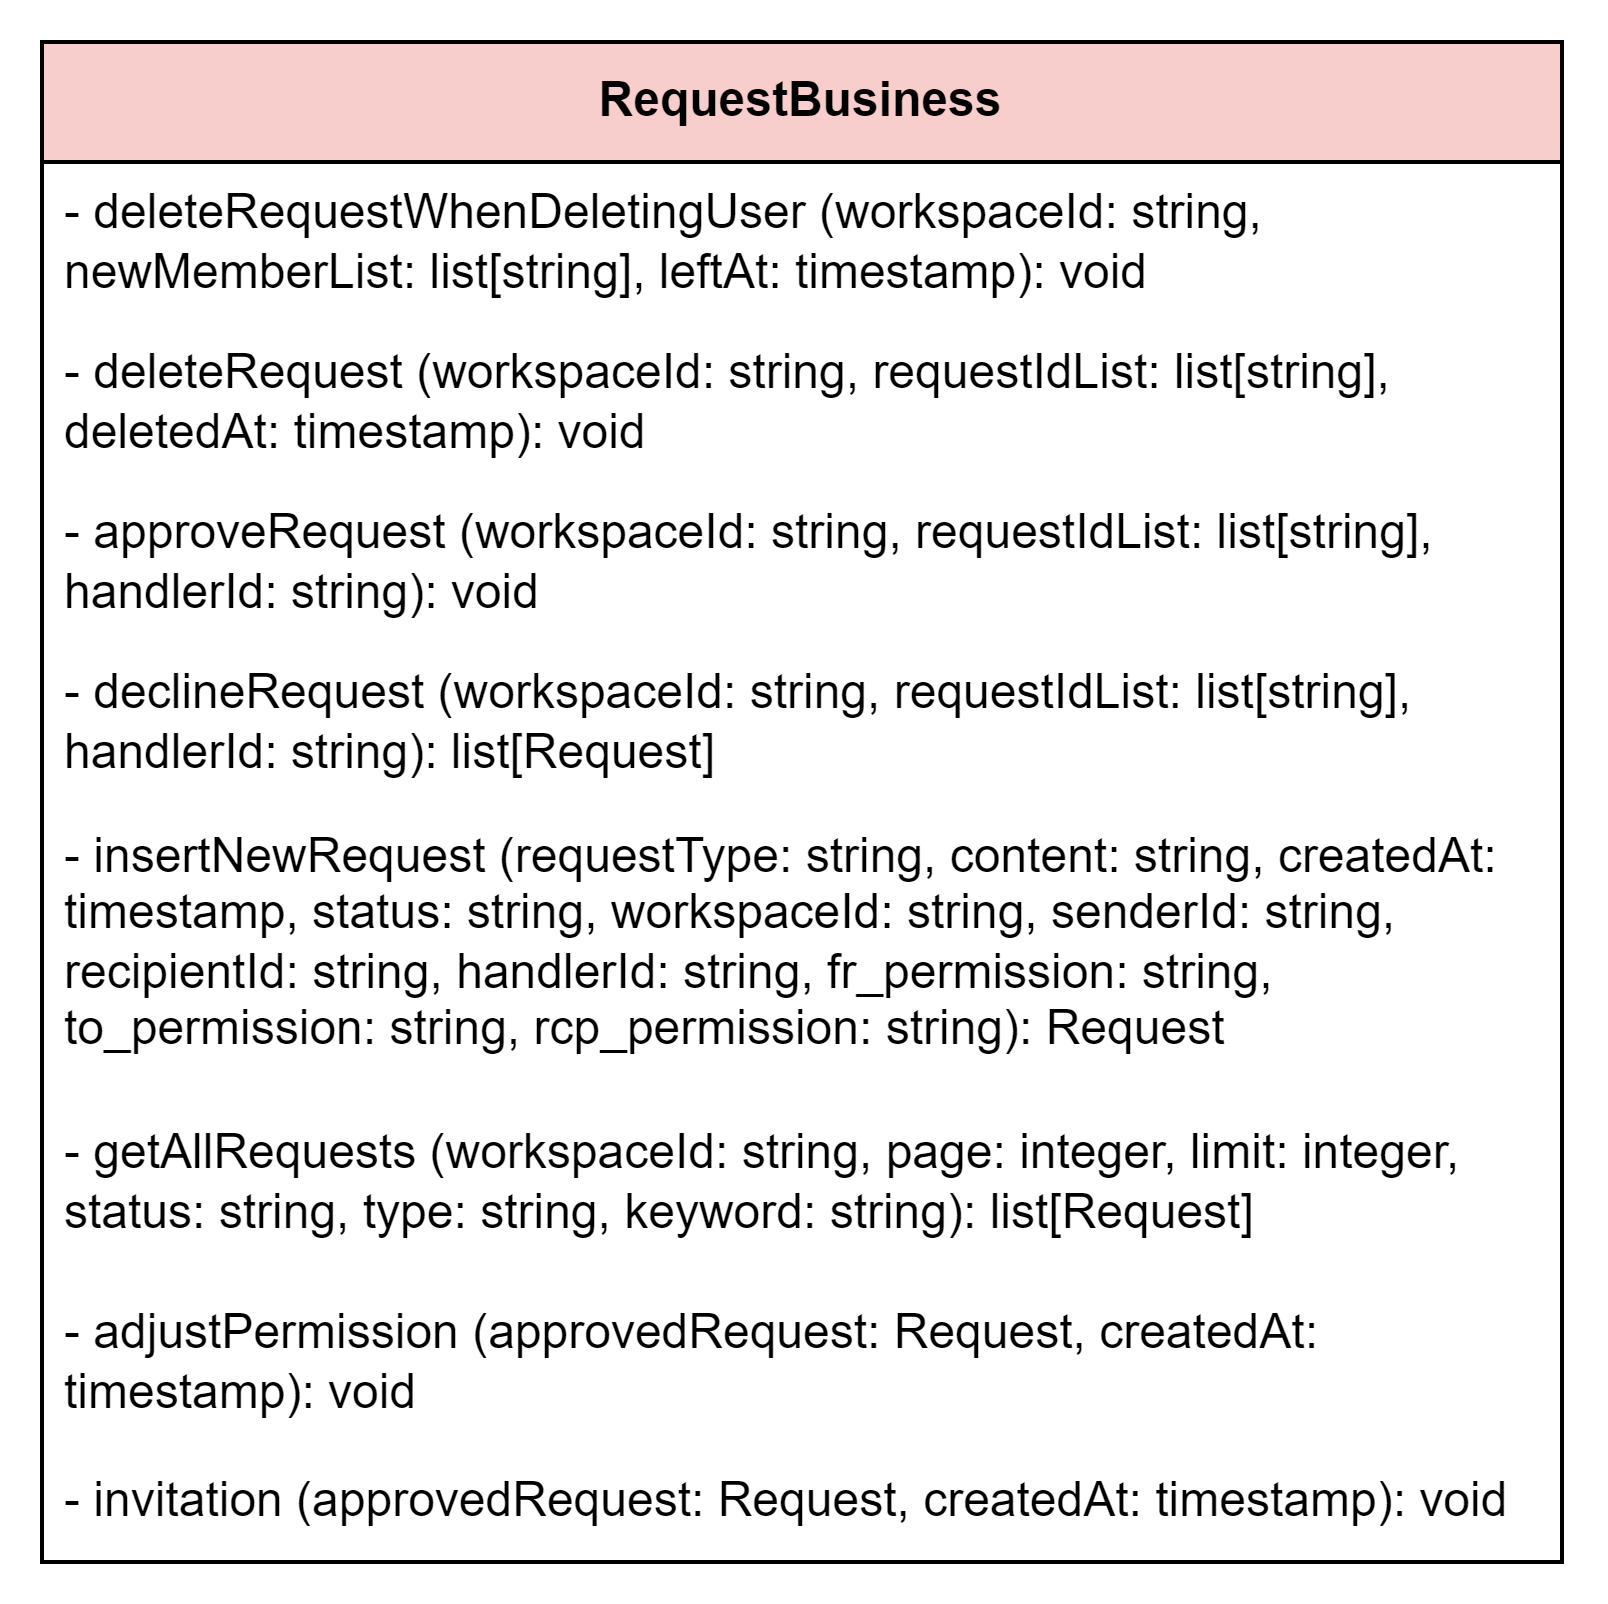
\includegraphics[ width = \linewidth]{Content/Phân tích và thiết kế hệ thống/documents/Sơ đồ lớp/images/Business layer/requestBusiness.png}
    \vspace{0.5cm}
    \caption{Class RequestBusiness trong Business layer}
    \label{fig:Class RequestBusiness trong Business layer}
\end{figure}
\par
Class RequestBusiness là class chịu trách nhiệm xử lý logic nghiệp vụ liên quan đến
những yêu cầu trong một Workspace. Class này sẽ thừa kế các class khác như:
Request\_Get\_Business, Request\_Delete\_Business, Request\_Update\_Business, Request\_Insert\_Business.
Những class này sẽ thực hiện các chức năng tương ứng với tên của chúng. Ngoài ra, class
Request\_Update\_Business còn kế thừa từ class Request\_Handling\_Business, class này sẽ thực
hiện chức năng xử lý những yêu cầu.
\begin{figure}[H]
    \centering
    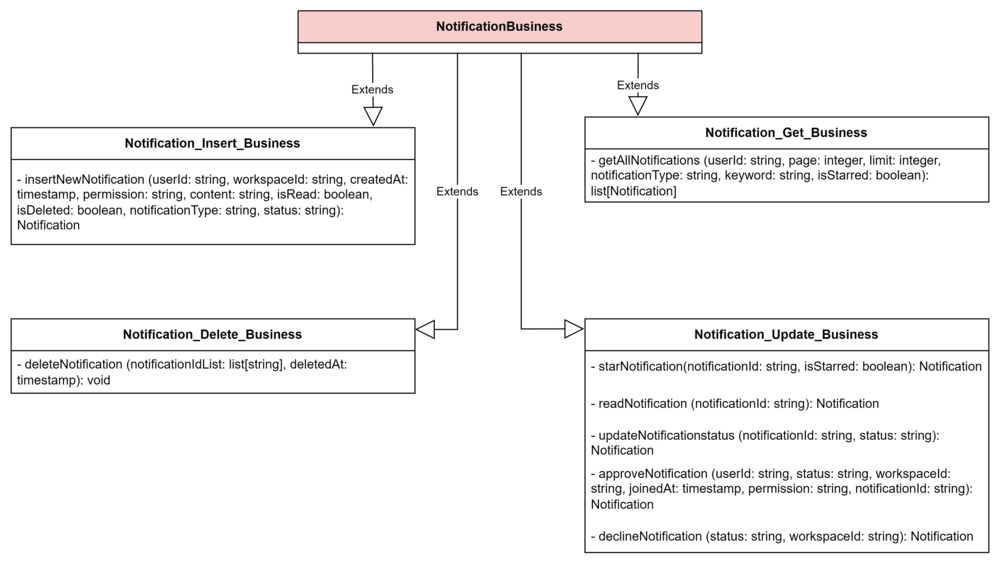
\includegraphics[ width = \linewidth]{Content/Phân tích và thiết kế hệ thống/documents/Sơ đồ lớp/images/Business layer/notificationBusiness.png}
    \vspace{0.5cm}
    \caption{Class NotificationBusiness trong Business layer}
    \label{fig:Class NotificationBusiness trong Business layer}
\end{figure}
\par
Class NotificationBusiness là class chịu trách nhiệm xử lý logic nghiệp vụ liên quan đến
những thông báo trong một Workspace. Tương tự như những class trên, class này sẽ thừa kế các class khác như:
Notification\_Get\_Business, Notification\_Delete\_Business, Notification\_Update\_Business, Notification\_Insert\_Busines.
